\documentclass[11pt,notes=hide,aspectratio=169]{beamer}
%Jonathan Dingel; PhD trade course

% PACKAGES
\usepackage{graphics}  % Support for images/figures
\usepackage{graphicx}  % Includes the \resizebox command
\usepackage{url}	   % Includes \urldef and \url commands
\usepackage{soul}      % Includes the underline \ul command
%\usepackage{framed}	   % Includes the \framed command for box around text
\usepackage{booktabs} %\toprule,\bottomrule
%\usepackage{natbib}
\usepackage{bibentry}  % Includes the \nobibliography command
\usepackage{bbm}       %
%\usepackage{pgfpages}  %Supports "notes on second screen" option for beamer
\usepackage{verbatim}  %Supports comments
\usepackage{tikz}		%Supports graphing/drawing
\usepackage{pgfplots} %Supports graphing/drawing
\usepackage{amsfonts}  % Lots of stuff, including \mathbb 
\usepackage{amsmath}   % Standard math package
\usepackage{amsthm}    % Includes the comment functions
\usepackage{physics}

% CUSTOM DEFINITIONS
\def\newblock{} %Get beamer to cooperate with BibTeX
\linespread{1.2}
\hypersetup{backref,pdfpagemode=FullScreen,colorlinks=true,linkcolor=blue,urlcolor=blue}
\newtheorem{proposition}{Proposition}
\newtheorem{assumption}{Assumption}
\newtheorem{condition}{Condition}

% IDENTIFYING INFORMATION
\title{Topics in Trade}
\author{Jonathan I. Dingel}
\date{Fall \the\year}

% BEAMER TEACHING STUFF
\setbeamertemplate{navigation symbols}{}  %Turn off navigation bar

% THEMATIC OPTIONS
\definecolor{columbiablue}{RGB}{185,217,235}  %Columbia blue defined at https://visualidentity.columbia.edu/branding
\definecolor{columbiadarkblue}{RGB}{0,48,135}  %Columbia dark blue defined at https://visualidentity.columbia.edu/branding
\setbeamercovered{transparent=5}
\setbeamercolor{frametitle}{fg=columbiadarkblue}
\setbeamercolor{item}{fg=columbiadarkblue}
\usefonttheme{serif}
\setbeamercolor{button}{bg = white,fg = columbiadarkblue}
\setbeamercolor{button border}{fg = columbiadarkblue}

\setbeamertemplate{footline}{\begin{center}\textcolor{gray}{Dingel -- Topics in Trade -- \semester -- Week 11 -- \insertframenumber}\end{center}}
\usepackage{appendixnumberbeamer}
\begin{document}
% -----------------------------------------
\begin{frame}[plain]
\begin{center}
\large
\textcolor{columbiadarkblue}{ECON G6905\\
Topics in Trade\\ 
Jonathan Dingel\\
\semester, Week 11}
\vfill 
\includegraphics[width=0.4\textwidth]{../images/Columbia_logo.png}
\end{center}
\end{frame}
% -----------------------------------------
\begin{frame}{Today: Skill-Biased Agglomeration}
Economic geography of human capital:
Where do skilled workers live and why?
\medskip
My goal today is to tackle four questions:
\begin{itemize}
	\item Why should we care about the spatial distributions of skills and sectors?
	\item How do we know that agglomeration is skill-biased?
	\item How should we characterize skills when modeling cities?
	\item What tools are relevant for building and estimating models?
\end{itemize}
\end{frame}
% -----------------------------------------
% -----------------------------------------
\begin{frame}{Spatial distributions of skills and sectors} 
Why should we care about the spatial distributions of skills and sectors?
\begin{enumerate}
	\item They vary a lot
	\item They covary with city characteristics
	\item They are often used as exogenous variation 
	\item They should help us understand how cities work
\end{enumerate}
\end{frame}
% -----------------------------------------
\begin{frame}{Spatial distributions of skills and sectors}
\begin{itemize}
	\item Public discussion describes US cities in terms of skills and sectors
	\item Ranking cities by educational attainment is a popular media exercise
	\begin{center}
\raisebox{-0.5\height}{\href{http://www.businessinsider.com/the-25-most-educated-cities-in-america-2014-9}{\includegraphics[width=0.45\textwidth]{../images/week10/mosteducatedcities_businessinsider.png}}}
	\raisebox{-0.5\height}{\href{http://www.marketwatch.com/story/the-10-smartest-cities-in-america-2015-01-02}{\includegraphics[width=0.45\textwidth]{../images/week10/smartestcities_marketwatch.png}}}
		\end{center}
	\item Place names are shorthand for sectors
	\begin{center}
	\raisebox{-0.5\height}{\includegraphics[width=0.3\textwidth]{../images/week10/wallstreetsign.jpeg}}
	\raisebox{-0.5\height}{\includegraphics[width=0.4\textwidth]{../images/week10/Silicon_valley_title.png}}
	\raisebox{-0.5\height}{\includegraphics[width=0.2\textwidth]{../images/week10/detroitbigthree.jpg}}
	\end{center}
\end{itemize}
\end{frame}
% -----------------------------------------
\begin{frame}{Educational attainment varies a lot across cities}
	\begin{center}
	Share of population 25 and older with bachelor's degree or higher
	\includegraphics[height=0.76\textheight]{../images/week10/CBSA_2009ACS_baplus_48states.pdf} \\
	\scriptsize{\textsc{Data source:} \href{http://www.census.gov/programs-surveys/acs/data.html}{American Community Survey}, 2005-2009, Series S1501
	\hfill \textsc{Plot:} CBSAs for \href{https://michaelstepner.com/maptile/}{maptile}}
	\end{center}
\end{frame}
% -----------------------------------------
\begin{frame}{Sectoral composition varies a lot across cities}
	\begin{center}
	Employment share of Professional, Scientific, and Technical Services
	\includegraphics[height=0.76\textheight]{../images/week10/CBSA_2009_techservicesshare.pdf}\\
	\scriptsize{\textsc{Data source:} \href{http://www2.census.gov/econ2009/CBP_CSV/}{County Business Patterns}, 2009, NAICS 54
	\hfill \textsc{Plot:} CBSAs for \href{https://michaelstepner.com/maptile/}{maptile}}
	\end{center}
\end{frame}
% -----------------------------------------
\begin{frame}{They covary with city characteristics}
	\begin{center}
	\only<1>{
	Populations of three educational groups across US metropolitan areas\\
	\includegraphics[height=.86\textheight]{../images/week10/CAC_figure1_edu.pdf}\\
	\vspace{-2mm}
	\scriptsize{\textsc{Data source:}  2000 Census of Population microdata via \href{https://usa.ipums.org/usa/}{IPUMS-USA}}
	}
	\only<2>{
	Employment in three occupations across US metropolitan areas\\
	\includegraphics[height=.86\textheight]{../images/week10/CAC_figure2_occ.pdf}\\
	\vspace{-2mm}
	\scriptsize{\textsc{Data source:} \href{http://www.bls.gov/oes/2000/oessrcma.htm}{Occupational Employment Statistics 2000}}
	}
	\only<3>{
	\includegraphics[width=.45\textwidth]{../images/week10/CAC_figure1_edu.pdf}
	\includegraphics[width=.45\textwidth]{../images/week10/CAC_figure2_occ.pdf}
	}
	\end{center}
\only<3>{
Skills and sectors are strongly linked to cities' sizes
\begin{enumerate}[(a)]
	\item Confounds inference: Agglomeration benefits vs compositional effects
	\item Confounds counterfactuals: Making NYC 10x larger raises finance's share of national employment and GDP
\end{enumerate}
}
\end{frame}
% -----------------------------------------
\begin{frame}{They are often used as exogenous variation}
It is common to see the following theory-empirics pairing:
\begin{itemize}
	\item Model: all locations produce a homogeneous good
	\item Estimation by shift-share design: exogenous shifts in local labor demand via local industrial composition $\times$ national changes in industrial employment
\end{itemize}
What variation does this shift-share design exploit?
\begin{itemize}
	\item \href{https://paulgp.github.io/papers/bartik_gpss.pdf}{GPSS}: employment shares are IVs measuring exposure to shifts
	\item \href{https://doi.org/10.1093/qje/qjz025}{AKM} \& \href{https://doi.org/10.1093/restud/rdab030}{BHJ}: sectoral shifters are randomly assigned and independent
	\item Skill mix vs industry mix (e.g., endogenous local SBTC of \href{http://www.jstor.org/stable/10.1086/658371}{Beaudry, Doms, Lewis 2010})
	\item City characteristics covarying with skills and sectors highlight exclusion-restriction assumptions 
%	\item 
\end{itemize}
\end{frame}
% -----------------------------------------
\begin{frame}{They should help us understand how cities work}
\begin{itemize}
	\item Why do different people and different businesses locate in different places?
	\item The answers should be crucial to understanding how cities work
\item Lucas (1988): ``the `force' we need to postulate account for the central role of cities in economic life is of exactly the same character as the `external human capital' I have postulated as a force to account for certain features of aggregative development.''
	\item Which elements of the Marshallian trinity imply we'll find finance and dot-coms in big cities?
	\item Coagglomeration (\href{https://www.aeaweb.org/articles.php?doi=10.1257/aer.100.3.1195}{Ellison Glaeser Kerr 2010}) and heterogeneous agglomeration (\href{https://ideas.repec.org/p/ehl/lserod/58426.html}{Faggio, Silva, Strange 2015}) can provide clues
	\item \href{https://www.conor-walsh.com/s/EGW.pdf}{Eckert, Ganapati, Walsh (2024)}: Wage growth since 1980 has been faster in larger cities and it's all in business services
\end{itemize}
\end{frame}
% -----------------------------------------
\begin{frame}{An introduction to skill-biased agglomeration}
\begin{itemize}
	\item Central fact:
Larger cities have 
higher college-graduate shares
\textcolor{gray}{(Berry \& Glaeser 2005, Moretti 2012)}
and
higher college wage premia
\textcolor{gray}{(Baum-Snow \& Pavan 2013, Davis \& Dingel 2019)}
\begin{center}
\includegraphics[width=.45\textwidth]{../images/week10/BaumSnowPavan2013fig3a.pdf}
\includegraphics[width=.45\textwidth]{../images/week10/BaumSnowPavan2013fig3b.pdf}\\
{ \footnotesize \href{http://www.mitpressjournals.org/doi/pdf/10.1162/REST_a_00328}{Baum-Snow and Pavan, ``Inequality and City Size'', 2013}}
\end{center}
\item How to explain spatial variation in relative prices and relative quantities?
\item {Start from ``canonical model'' with two skill types and spatial variation in relative supply and relative demand\par}
\end{itemize}
\end{frame}
% -----------------------------------------
\begin{frame}{Spatial equilibrium with two skill groups}
A simple starting point
\begin{enumerate}
	\item Two skill groups, $s \in \{L,H\}$
	\item Elastic labor supply: $U_s(A_c,w_{s,c},p_{c}) = U_s(A_{c'},w_{s,c'},p_{c'}) \ \forall c,c' \ \forall s$
	\item Homothetic preferences: $U_s(A_{c},w_{s,c},p_{c}) = \frac{w_{s,c} A_{c}}{p_{c}}$
\end{enumerate}
\medskip \pause 
These jointly imply that relative wages are spatially invariant:
\begin{align*}
\frac{w_{H,c} A_{c}}{ p_{c}} = \frac{w_{H,c'}A_{c'}}{p_{c'}} 
\quad&\textnormal{ and }\quad 
\frac{w_{L,c} A_{c}}{p_{c}} = \frac{w_{L,c'}A_{c'} }{p_{c'}} \\
\implies \frac{w_{H,c}}{w_{L,c}} &= \frac{w_{H,c'}}{w_{L,c'}} \ \forall c,c'
\end{align*}
\end{frame}
\begin{frame}{Spatial equilibrium and skill premia (two types; homothetic prefs)}
\begin{center}\vspace{-2mm}
\begin{tikzpicture}[range=0:200,scale=1.0,thick,font=\normalsize]
\begin{axis}[
	xmin=0, 
	xmax=10,
	ymin=0,
	ymax=10,
	xticklabels=\empty,
	yticklabels=\empty,
	clip=false,
	axis lines=left,
	xtick=\empty,
	ytick=\empty,
]
% Curves
\addplot [black, line width = 1, smooth, domain=1:8.5] {9.5 - x} node[right,color=black,align=left]{Relative demand};
\only<1>{\addplot [black, line width = 1, smooth, domain=0:10] {5} node[right,color=black,align=left]{Relative supply \\ Rosen(1979), Roback(1982)};}
\only<2>{\addplot [black, line width = 1, smooth, domain=0:9] {x} node[right,color=black,align=left]{Relative supply \\ Topel (1986), Moretti (2011),\\ Diamond (2016)};}
\only<3>{\addplot [black, line width = 1, smooth, domain=0:9] {x} node[right,color=white,align=left]{Relative supply \\ Topel (1986), Moretti (2011),\\ Diamond (2016)};}
\only<3>{\addplot [red, line width = 1, smooth, domain=1:9] {11 - x} node[right,color=black,align=left]{Skill-biased agglomeration};}
% Labels
\node [below] at (current axis.right of origin) {${Q_H}/{Q_L}$};
\node [left] at (current axis.above origin) {${w_H}/{w_L}$};
\end{axis}
\end{tikzpicture}
\end{center}
\vspace{-3mm}
\only<1>{\scriptsize
	Differences in productivity ``tend to show up exclusively in changes in quantities of skilled people, not in different returns to skilled people across space'' (Glaeser 2008)
\par}
\only<1>{}
\end{frame}
% -----------------------------------------
\begin{frame}{Why not a story about relative supply?}
Preferences are not homothetic.
What happens if we relax that assumption?
\smallskip
Relative prices of income-elastic goods are lower in larger cities:
\begin{itemize}
\item Income elasticity of housing demand is less than one:\\
\href{https://www.nber.org/papers/w22816}{Albouy, Ehrlich, and Liu (2016)}, \href{https://trevorcwilliams.github.io/files/submission_fw.pdf}{Finlay and Williams (2023)}
\item Larger cities specialize in producing income-elastic tradable goods:\\
\href{https://doi.org/10.1093/restud/rdw054}{Dingel (2017)}, \href{https://doi.org/10.3982/ECTA11738}{Handbury (2021)}, \href{https://www.tksonoda.com/}{Onoda (2023)}
\end{itemize}
These are empirically relevant forces,
but they increase the relative supply of skill in larger cities
\end{frame}
% -----------------------------------------
\begin{frame}{Spatial equilibrium and skill premia (two types)}
\begin{center}
\vspace{-3mm}
\begin{tikzpicture}[range=0:200,scale=1.0,thick,font=\normalsize]
\begin{axis}[
	xmin=0, xmax=10, ymin=0, ymax=10, xticklabels=\empty, yticklabels=\empty, clip=false, axis lines=left, xtick=\empty, ytick=\empty,
]
% Curves
\addplot [black, line width = 1, smooth, domain=1:8.5] {9.5 - x} node[right,color=black,align=left]{Relative demand};
\only<2>{\addplot [red, line width = 1, smooth, domain=2:9] {12 - x} node[right,color=black,align=left]{Skill-biased agglomeration};}
\only<1>{
\addplot [black, line width = 1, smooth, domain=0:10] {6} node[right,color=black,align=left]{Relative supply};
\addplot [blue, line width = 1, smooth, domain=0:10] {4} node[right,color=black,align=left]{Big-city relative supply\\(BKT 2009, Lee 2010)};
}
\only<2>{
\addplot [black, line width = 1, smooth, domain=0:9] {x} node[right,color=black,align=left]{Relative supply};
\addplot [blue, line width = 1, smooth, domain=1:9] {x-1} node[right,color=black,align=left]{Big-city relative supply};
}
% Labels
\node [below] at (current axis.right of origin) {${Q_H}/{Q_L}$};
\node [left] at (current axis.above origin) {${w_H}/{w_L}$};
\only<1>{\node [right] at (50,85) {$ \frac{w_{H,c}}{P_{H,c}} = \frac{w_{H,c'}}{P_{H,c'}} , \frac{w_{L,c}}{P_{L,c}} = \frac{w_{L,c'}}{P_{L,c'}} , P_{H,c} \neq P_{L,c} $};}
\end{axis}
\end{tikzpicture}
\end{center}
\vspace{-5mm}
\only<1>{\footnotesize Black, Kolesnikova, Taylor (2009): ``if the income elasticity of housing is less than one\dots the return to education is lower in cities that are more expensive''\par}
\only<2>{With two types, the explanation for spatial variation in relative prices and relative quantities
lies in skill-biased agglomeration shifting relative demand.\par}
\end{frame}
% -----------------------------------------
\begin{frame}{What is skill-biased agglomeration?}
The canonical model is one way of interpreting the central fact
\begin{itemize}
	\item In two-type model,
larger cities have higher relative demand for skill
\item With more than two underlying types,
these relative quantities and relative prices may reflect compositional differences (i.e., spatial sorting)
\item I read the available empirical evidence as saying two types are not enough
\end{itemize}
\end{frame}
% -----------------------------------------
\begin{frame}{Two types in theory and practice}
Two-type models can be simple -- but what about two-type empirics?
\begin{itemize}
	\item Omit types: Davis \& Dingel (2019) plot of college wage premia shows bachelor's vs HS diplomas -- use only 45\% of population to test price prediction
	\item Convert quantities to ``equivalents'': ``one person with some college is equivalent to a total of 0.69 of a high school graduate and 0.29 of a college graduate'' (\href{http://www.jstor.org/stable/2118323}{Katz \& Murphy 1992}, p.68)
\end{itemize}
\pause Results may be sensitive to dichotomous definitions
\begin{itemize}
	%\item Berry \& Glaeser (2005): ``US metropolitan areas with more college graduates in 1990 became increasingly skilled over the 1990s''
	\item \href{https://www.aeaweb.org/articles?id=10.1257/aer.20131706}{Diamond (2016)}: ``A MSA's share of college graduates in 1980 is positively associated with larger growth in its share of college workers from 1980 to 2000''
	\item \href{https://www.aeaweb.org/articles?id=10.1257/app.20160510}{Baum-Snow, Freedman, Pavan (2015)}: ``Diamond's result does not hold for CBSAs if those with some college education are included in the skilled group.''
\end{itemize}
\end{frame}
% -----------------------------------------
\begin{frame}{Dichotomous approach misses relevant variation}
\begin{itemize}
	\item In labor economics, the canonical two-skill model ``is largely silent on a number of central empirical developments of the last three decades'', such as wage polarization and job polarization (\href{http://www.sciencedirect.com/science/article/pii/S0169721811024105}{Acemoglu and Autor 2011})
	\item In the urban context, there is systematic variation across cities in terms of finer observable categories: population elasticities for high school graduates (.925), associate's degree (0.997), bachelor's degree (1.087), and professional degree (1.113) (\href{https://doi.org/10.1016/j.jinteco.2020.103291}{Davis and Dingel 2020})
\end{itemize}
\end{frame}
% -----------------------------------------
\begin{frame}{How much should we worry about spatial sorting?}
Contrasting views.
Suggestions of sorting:
\begin{itemize}
	\item  {\small ``Workers in cities with a well-educated labor force are likely to have unobserved characteristics that make them more productive than workers with the same level of schooling in cities with a less-educated labor force. For example, a lawyer in New York is likely to be different from a lawyer in El Paso, TX.'' (\href{https://ideas.repec.org/h/eee/regchp/4-51.html}{Moretti 2004, p.2246})\par}
	\item {Within occupations, job postings in larger cities require more interactive tasks and using newer technologies, especially for college graduates (\href{http://www-personal.umich.edu/~ssotelo/research/AST_geography.pdf}{Atalay, Sotelo, Tannenbaum 2021})}
	\end{itemize}
Claim of little sorting (e.g., \href{http://diegopuga.org/research/dreams.pdf}{de la Roca, Ottaviano, Puga 2023}) stems from:
\begin{itemize}
	\item Cognitive test scores in NLSY79 (11,000 US individuals)
	\item Estimated finite-mixture model using NLSY79 (\href{https://ideas.repec.org/a/oup/restud/v79y2012i1p88-127.html}{Baum-Snow \& Pavan 2012})
\item Individual fixed effects from AKM-style regressions
\end{itemize}
\end{frame}
% -----------------------------------------
\begin{frame}{Evidence of little spatial sorting from US NLSY79}
National Longitudinal Survey of Youth 1979 (NLSY79)
\begin{itemize}
	\item \href{http://econpapers.repec.org/article/eeejuecon/v_3a65_3ay_3a2009_3ai_3a2_3ap_3a136-153.htm}{Bacolod, Blum, Strange (2009)}: ``The mean AFQT scores do not vary much across [four] city sizes'' within occupational categories
	\item BBS observe only one sales person in MSAs with 0.5m -- 1.0m residents (10th and 90th percentiles of AFQT are equal) \hyperlink{BBS2009tab5}{\beamergotobutton{table}}
	\item \href{https://ideas.repec.org/a/oup/restud/v79y2012i1p88-127.html}{Baum-Snow \& Pavan (2012)}: Estimated finite-mixture model implies ``sorting on unobserved ability within education group\dots contribute little to observed city size wage premia.''
	\item BSP use NLSY79 data on 1754 white men; 583 have bachelor's degree or more; college wage premia don't rise with city size \hyperlink{BSPvsCensus}{\beamergotobutton{table}}
\end{itemize}
\hypertarget{NLSY_main}{}
\end{frame}
% -----------------------------------------
\begin{frame}{Bringing more US data to bear on sorting}
\begin{itemize}
	\item \href{https://nces.ed.gov/surveys/b&b/}{Baccalaureate and Beyond} tracks a cohort graduating from four-year colleges in 1993 
	\item In 2003, look at 2,300 white individuals who obtained no further education after bachelor's degree and now live in a MSA
	\item Look at variation in SAT scores across cities -- all variation is within the finest age-race-education cell in typical public data sets
	\item Mean SAT score in metros with more than 3.25m residents is 40 points higher than metros with fewer than 0.57m residents
\end{itemize}
\end{frame}
% -----------------------------------------
\begin{frame}{Sorting within observable demographic cells}
\begin{itemize}
	\item Mean SAT score in metros with more than 3.25m residents is 40 points higher than metros with fewer than 0.57m residents
	\item Full distribution suggests stochastic dominance
	\begin{center}\includegraphics[height=.70\textheight]{../images/week10/SATscore3_trimmed.pdf}\end{center}
\end{itemize}
\end{frame}
% -----------------------------------------
\begin{frame}{Evidence from wage regressions with worker fixed effects}
\href{https://academic.oup.com/restud/article/84/1/106/2669971}{de la Roca and Puga (2017)}
use Spanish tax data on 2004-2009 earnings:
\begin{itemize}{
	\item 157,113 workers and 40,809 cross-city moves
	\item Assume random migration conditional on observables
	\item $e_{ijt}$ is worker $i$'s experience in city $j$ through time $t$
\item Estimating equation:
\begin{equation*}
\ln w_{ict} = \sigma_c + \mu_i + \sum_{j=1}^{C} \delta_{jc} e_{ijt} + \beta x_{it} + \epsilon_{ict}
\end{equation*}
\item
If one only estimates a static specification
\begin{equation*}
\ln w_{ict} = \sigma_c + \mu_i  + \beta x_{it} + \zeta_{ict}
\end{equation*}
$\hat{\sigma}_{c}$ may be biased if
$\text{Cov}\left((\iota_{ict} - \bar{\iota}_{ic}),\sum_{j}^{C} \delta_{jc} (e_{ijt} - \bar{e}_{ij})\right) \neq 0$
(if workers' experience is higher when they are in $c$)
}\end{itemize}
\end{frame}
% -----------------------------------------
\begin{frame}{de la Roca and Puga (2017) on dynamics and sorting}
\begin{itemize}
\item Experience in larger cities is more valuable and portable
\only<1>{
	\begin{center}
	Earnings of equivalent workers in Madrid (largest) and Sevilla (fourth largest) relative to Santiago de Compostela (median)\\
	\includegraphics[height=0.75\textheight]{../images/week10/delaRocaPuga2017_fig3a.pdf}
	\end{center}
}
\only<2->{\item Big-city experience is more valuable for workers with higher ability}
\only<2>{
	\begin{center}
	\includegraphics[height=0.75\textheight]{../images/week10/delaRocaPuga2017_fig7.pdf}
	\end{center}
}
\only<3->{\item There is sorting across five occupational categories}
\only<3>{
	\begin{center}
	\includegraphics[width=0.9\textwidth]{../images/week10/delaRocaPuga2017_tab5.pdf}
	\end{center}
}
\only<4->{\item Little sorting within these categories when using full dynamic specification
\begin{center}
	\includegraphics[height=0.55\textheight]{../images/week10/delaRocaPuga2017_fig8c.pdf}
	\includegraphics[height=0.55\textheight]{../images/week10/delaRocaPuga2017_fig8a.pdf}
\end{center}
}
\end{itemize}
\only<4->{}
\end{frame}
% -----------------------------------------
\begin{frame}{Norweigan wage regressions with worker fixed effects}
\href{https://doi.org/10.1016/j.regsciurbeco.2016.06.006}{Carlsen Ratts\o\ \& Stokke (2016)}
use 2003-2010 data on Norway:
\begin{itemize}
\item
College-educated workers have higher return to big-city experience
\item
The city wage premium trajectories depend on job tenure
\only<1>{\begin{center}\includegraphics[height=0.6\textheight]{../images/week10/CarlsenRattsoStokke2016_fig1.pdf}\end{center}}
\only<2>{
\item
Sorting on unobserved abilities is driven by the college educated
\begin{center}
\includegraphics[height=0.5\textheight]{../images/week10/CarlsenRattsoStokke2016_fig2b.pdf}
\includegraphics[height=0.5\textheight]{../images/week10/CarlsenRattsoStokke2016_fig2c.pdf}
\end{center}
\item
{Sorting by young: no sorting on worker fixed effects among older workers\par}
}
\end{itemize}
\end{frame}
% -----------------------------------------
\begin{frame}{US wage regressions with worker fixed effects}
\href{https://www.nber.org/papers/w31587}{Card, Rothstein, Yi (2023)}
use Longitudinal Employer-Household Dynamics data:
\begin{itemize}{
\item Abowd-Kramarz-Margolis wage regression with worker FEs, establishment FEs, and controls for age and time
\item Commuting Zone effect is average of establishment FEs in the CZ
(specification with worker FEs and CZ FEs biased by ``hierarchy effect'')
\item {\small ``We find some evidence of the kind of dynamic returns to `big city' experience highlighted by de la Roca and Puga (2017) but the addition of this channel has little impact on the static returns to different CZs''\par}
\item Half of the observed large-CZ earnings premium reflects worker sorting
\item 2/3 of spatial variation in college wage premia is variation in relative skills
\item Much of the remaining 1/3 is because of enhanced sorting of college-educated workers to high-wage industries in larger CZs
}\end{itemize}
\end{frame}
% -----------------------------------------
\begin{frame}{Modeling a spatial economy with a continuum of skills}
Why work with a continuum?
\begin{itemize}
	\item Evidence for sorting on characteristics that are typically not observed
	\item Need at least five types to capture sorting on observables in the sense of de la Roca and Puga (2017)
	\item Modeling a finite, particular number of types is potentially painful
\end{itemize}
Continuum case can be quite tractable
\begin{itemize}
	\item See \href{https://ideas.repec.org/a/ucp/jpolec/doi10.1086-675534.html}{Behrens, Duranton, Robert-Nicoud (2014)}, \href{http://www.jdingel.com}{Davis and Dingel (2019, 2020)}, \href{http://www.sciencedirect.com/science/article/pii/B9780444595171000040}{Behrens and Robert-Nicoud (\emph{Handbook} 2015)}
	\item These papers rely on tools from the assignment literature
	\item Assignments of individuals/firms to cities, with endogenous city characteristics determined in equilibrium
	\item Davis and Dingel (2020) speak to both skills and sectors
\end{itemize}
\end{frame}
% -----------------------------------------
\begin{frame}{ Davis \& Dingel - A Spatial Knowledge Economy (2019)}
We have models of: 
\begin{itemize}
	\item Knowledge spillovers as a pure externality (one interpretation of Henderson 1974, Black 1999, Lucas 2001)
	\item Endogenous exchange of ideas in a single (or symmetric) location(s) (Helsley and Strange 2004, Berliant, Reed III, and Wang 2006, Berliant and Fujita 2008, Lucas and Moll 2014)
\end{itemize}
Our contribution:
\begin{itemize}
	\item Introduce a model of a system of cities in which costly idea exchange is the agglomeration force 
	\item Our model replicates a broad set of facts about the cross section of cities
	\item We provide a spatial-equilibrium explanation of why skill premia are higher in larger cities and how this emerges from symmetric fundamentals
\end{itemize}
\end{frame}
% -----------------------------------------
\begin{frame}{Model summary}
Our model's core components: 
\begin{itemize}
\item Spatial equilibrium -- zero mobility costs 
\item Heterogeneous workers -- continuum of abilities 
\item Two sectors: 
\begin{itemize}
	\item Tradables: Labor heterogeneity matters for productivity
	\item Non-tradables: Homogeneous productivity
\end{itemize}
\item Skilled tradables sector has local learning opportunities 
\begin{itemize}
	\item Workers choose to spend time exchanging ideas 
	\item Gains from interactions increasing in own ability and peers' ability
\end{itemize}
\item Congestion costs make housing more expensive in larger cities 
\item Workers choose locations, occupations, and time spent exchanging ideas 
\end{itemize}
\end{frame}
% -----------------------------------------
\begin{frame}{Preferences and congestion}
\begin{itemize}
	\item Preferences: Unit demand for housing and $\bar{n}$-unit demand for non-tradable:
	\begin{equation*}
	V(p_{n,c},p_{h,c},y)= y-p_{n,c}\bar{n}-p_{h,c}. \label{indirect_utility}
	\end{equation*}
	\item Each individual in a city of population $L_c$ pays a net urban cost (in units of the numeraire) of 
	\begin{equation*}
	p_{h,c} = \theta L_c^\gamma
	\end{equation*}
	\item Individuals are perfectly mobile across cities and jobs, so their locational and occupational choices maximize $V(p_{n,c},p_{h,c},y)$.
\end{itemize}
\end{frame}
% -----------------------------------------
\begin{frame}{Production}
\begin{itemize}
	\item An individual can produce tradables ($t$) or non-tradables ($n$)
	\item An individual working in sector $\sigma$ earns income equal to the value of her output, which is
		\begin{equation*}
		y =  \Bigg\{\begin{array}{cc}
		p_{n,c} & \textnormal{ if } \sigma = n \\
		\tilde{z}(z,{Z}_{c})  & \textnormal{ if } \sigma = t \end{array}
		\end{equation*}
	\item Tradables production depends on own ability $(z)$, time spent producing ($\beta$), time spent exchanging ideas ($1-\beta$), and local learning opportunities $(Z_{c})$:
		\begin{equation*}
		\tilde{z}(z,Z_c) = \max_{\beta\in[0,1]} B(1-\beta,z,Z_c)
		\end{equation*}
\end{itemize}
\end{frame}
% -----------------------------------------
\begin{frame}{Idea exchange}
Tradables production:
		\begin{equation*}
		\tilde{z}(z,Z_c) = \max_{\beta\in[0,1]} B(1-\beta,z,Z_c)
		\end{equation*}
\begin{itemize}
\item Scalar $Z_c$ depends on time-allocation decisions of all agents in $c$. 
\item Denote idea-exchange time of ability $z$ in city $c$ by $1-\beta_{z,c}$ 
\item Denote local ability distribution $\mu(z,c)$, where $\frac{\mu(z,c)}{\mu(z)}$ is the share of $z$ in $c$.
		\begin{equation*}
		Z_c = Z(\{1-\beta_{z,c}\},\{\mu(z,c)\}). \label{eqn:bigZfunction}
		\end{equation*}
\item Denote total time devoted to learning by tradables producers in city $c$ by $M_c$
\begin{equation*}
M_{c} = L \int_{z: \sigma(z)=t}(1-\beta_{z,c})\mu(z,c) dz.
\end{equation*}
\end{itemize}
\end{frame}
% -----------------------------------------
\begin{frame}{Idea exchange: General assumptions}
\begin{itemize}
{\small
\item \textbf{Assumption 1}. 
The production function for tradables
$B(1-\beta,z,Z_c)$ is continuous,
strictly concave in $1-\beta$,
strictly increasing in $z$, and increasing in $Z_c$.
$B(1-\beta,z,0)=\beta z$ and $B(0,z,Z_c)=z$ $\forall z$.
\item \textbf{Assumption 2}. 
Tradables output $\tilde{z}(z,Z_c)$ is supermodular and
is strictly supermodular on $\otimes \equiv \{(z,Z): \tilde{z}(z,Z)>z\}$.
\item \textbf{Assumption 3}. 
The idea-exchange functional
$Z(\{1-\beta_{z,c}\},\{L\cdot\mu(z,c)\})$
is continuous, equal to zero if $M_c=0$, and bounded above by $\sup \{z:1-\beta_{z,c}>0,\mu(z,c)>0\}$.
If  $M_{c} > M_{c'}$ and $\{(1-\beta_{z,c})\mu(z,c)\}$ stochastically dominates $\{(1-\beta_{z,c'})\mu(z,c')\}$,
then $Z(\{1-\beta_{z,c}\},\{L\cdot\mu(z,c)\})>Z(\{1-\beta_{z,c'}\},\{L\cdot\mu(z,c')\})$.
}
\end{itemize}
\end{frame}
% -----------------------------------------
\begin{frame}{Idea exchange: Special case}
For some of our analysis, we focus on particular functional forms for $B(\cdot)$ and $Z(\cdot)$:
\begin{align*}
&B(1-\beta,z,Z_c) = {\beta}z(1+(1-\beta)A{Z}_{c}z) \\
&Z(\{(1-\beta_{z,c}),\mu(z,c)\})  = \left(1-\exp(-\nu M_c) \right) \bar{z}_{c} \\
\bar{z}_{c} & =\Bigg\{\begin{array}{cc}
\int_{z: \sigma(z)=t}\frac{(1-\beta_{z,c})z}{\int_{z: \sigma(z)=t}(1-\beta_{z,c})\mu(z,c) dz}\mu(z,c) dz & \textnormal{ if }M_{c}>0\\
0 & \textnormal{ otherwise } \nonumber
\end{array} 
\end{align*}
\begin{itemize}
	\item Random matching: Probability of encounter during each moment of time spent seeking idea exchanges is $\left(1-\exp(-\nu M_c) \right)$
	\item $M_{c}$ is the total time devoted to idea exchange
	\item $\bar{z}_{c}$ is the average ability of the individuals encountered
\end{itemize}
\end{frame}
% -----------------------------------------
\begin{frame}{Two lemmas}
\begin{lemma}[Comparative advantage]
\label{lemma:ComparativeAdvantage}
Suppose that Assumption 1 holds. There is an ability level $z_m$ such that individuals of greater ability produce tradables and individuals of lesser ability produce non-tradables. 
\begin{align*}
\sigma(z) =  \Bigg\{\begin{array}{cc}
t & \textnormal{ if } z > z_m \\
n & \textnormal{ if } z < z_m \end{array}
\end{align*}
\end{lemma} 
\begin{lemma}[Spatial sorting of tradables producers engaged in idea exchange]\label{lemma:spatialsorting}
Suppose that Assumption 2 holds. For $z>z'>z_m$, if $\mu(z,c)>0$, $\mu(z',c')>0$, $\beta(z,Z_{c})<1$, and $\beta(z',Z_{c'})<1$, then $Z_c \geq Z_{c'}$.
\end{lemma}
\end{frame}
% -----------------------------------------
\begin{frame}{Spatial equilibrium}
\begin{proposition}[Heterogeneous cities' characteristics] \label{prop:crosscitycharacteristics}
Suppose that Assumptions 1 and 2 hold. In any equilibrium, a larger city has higher housing prices, higher non-tradables prices, a better idea-exchange environment, and higher-ability tradables producers. If $L_c > L_{c'}$ in equilibrium, then $p_{h,c}>p_{h,c'}$, $p_{n,c}>p_{n,c'}$, $Z_c>Z_{c'}$, and $z>z'>z_m \Rightarrow$ $\mu(z,c)\mu(z',c')\geq\mu(z,c')\mu(z',c)=0$.
\end{proposition}
\end{frame}
% -----------------------------------------
\begin{frame}{Spatial equilibrium: Two-city example}
\begin{center}
\includegraphics[height=0.9\textheight]{../images/week10/SKE_2citywageschedule.pdf}
\end{center}
\end{frame}
% -----------------------------------------
\begin{frame}{Differences in average wages}
\begin{itemize}
	\item Differences in tradables producers' wages are the sum of three components: composition, learning, and compensation effects
	\item Denote $z_b$ the ``boundary'' ability of indifferent tradables producer
	\item Define inframarginal learning $\Delta(z,c,c')\equiv\left[\tilde{z}(z,Z_{c})-\tilde{z}(z,Z_{c'})\right]-\left[\tilde{z}(z_{b},Z_{c})-\tilde{z}(z_{b},Z_{c'})\right]$
	\item Define the density of tradables producers' abilities in city $c$ by $\tilde{\mu}(z,c)\equiv\frac{\mu(z,c)}{\int_{z':\sigma(z')=t}\mu(z',c)dz'}$
\end{itemize}
\begin{align*}%\left[\Delta(z,c,c')\right] became \Delta(z,c,c')
\bar{w}_{c}-\bar{w}_{c'} 
&
\equiv \frac{\int_{z:\sigma(z)=t}\tilde{z}(z,Z_{c})\mu(z,c)dz}{\int_{z:\sigma(z)=t}\mu(z,c)dz}-\frac{\int_{z:\sigma(z)=t}\tilde{z}(z,Z_{c'})\mu(z,c')dz}{\int_{z:\sigma(z)=t}\mu(z,c')dz} 
\\
& 
=\underbrace{\int_{z_m}^{\infty}[\tilde{\mu}(z,c)-\tilde{\mu}(z,c')]\tilde{z}(z,Z_{c'})dz}_{\textnormal{composition}} + \underbrace{\int_{z_m}^{\infty}\tilde{\mu}(z,c)\Delta(z,c,c')dz}_{\textnormal{inframarginal learning}} 
%&
\quad +\underbrace{p_{n,c}-p_{n,c'}}_{\textnormal{compensation}}
\end{align*}
\end{frame}
% -----------------------------------------
\begin{frame}{Skill premia}
\begin{itemize}
	\item Define a city's observed skill premium as its average tradables wage divided by its (common) non-tradables wage, $\frac{\bar{w}_{c}}{p_{n,c}}$
	\item When a tradables producer of ability $z_b$ is indifferent between cities $c$ and $c'$, this skill premium is higher in $c$ if and only if
\end{itemize}
\begin{equation*} %\left[\Delta(z,c,c')\right] became \Delta(z,c,c')
\underbrace{\int_{z_m}^{\infty}[\tilde{\mu}(z,c)-\tilde{\mu}(z,c')]\tilde{z}(z,Z_{c'})dz}_{\textnormal{composition}}
+\underbrace{\int_{z_m}^{\infty}\tilde{\mu}(z,c)\Delta(z,c,c')dz}_{\textnormal{inframarginal learning}}
\geq \underbrace{\left(p_{n,c}-p_{n,c'}\right)\left(\frac{\bar{w}_{c'}}{p_{n,c'}}-1\right)}_{\textnormal{relative compensation}}\label{eqn:premia_decomp}
\end{equation*}
\begin{itemize}
	\item Helpful to define a production-function property: 
	\begin{condition}\label{condition:outputelasticity}
	The ability elasticity of tradable output,
	$\frac{\partial\ln\tilde{z}\left(z,Z_{c}\right)}{\partial\ln z}$,
	is non-decreasing in $z$ and $Z_{c}$.
	\end{condition}
\end{itemize}
\end{frame}
% -----------------------------------------
\begin{frame}{Larger cities have higher skill premia}
\begin{proposition}[Skill premia] \label{prop:skillpremia}
Suppose that Assumptions 1 and 2 hold.
In an equilibrium in which the smallest city has population $L_{1}$ and the second-smallest city has population $L_{2}>L_{1}$,
\begin{enumerate}
\item if the ability distribution is decreasing, $\mu'(z)\leq0$, $\tilde{z}(z,Z_{c})$ is log-convex in $z$, and $\tilde{z}(z,Z_{c})$ is log-supermodular, then $\frac{\bar{w}_{2}}{p_{n,2}}>\frac{\bar{w}_{1}}{p_{n,1}}$;
\item if the ability distribution is Pareto, $\mu(z)\propto z^{-k-1}$ for $z\geq z_{\min}$ and $k>0$, and the production function satisfies Condition \ref{condition:outputelasticity}, then $\frac{\bar{w}_{2}}{p_{n,2}}>\frac{\bar{w}_{1}}{p_{n,1}}$;
\item if the ability distribution is uniform, $z\sim U\left(z_{\min},z_{\max}\right)$, the production function satisfies Condition \ref{condition:outputelasticity}, and $\frac{L_2 - L_1}{L_1^2} > \frac{1}{L}\frac{(1-\bar{n})(z_{\max} - z_{\min})}{z_{\min} +\bar{n}(z_{\max} - z_{\min})}$, then $\frac{\bar{w}_{2}}{p_{n,2}}>\frac{\bar{w}_{1}}{p_{n,1}}$.
\end{enumerate}
\end{proposition}
\end{frame}
% -----------------------------------------
\begin{frame}{Larger cities have higher skill premia}
\begin{itemize}
	\item The three cases in Proposition 2 trade off stronger assumptions about the production function with weaker assumptions about the ability distribution
	\item Paper contains numerical results for more than two cities for special case of
	$B(1-\beta,z,Z_c) = {\beta}z(1+(1-\beta)A\left(1-\exp(-\nu M_c) \right) \bar{z}_{c} z)$
	\item Paper contains illustrative example with 275 cities that quantitatively matches Zipf's law, premia-population correlation, and size-invariant housing expenditure shares
\item Numerical comparative static: 10\% increase in $A$ leaves the power-law exponent virtually unchanged and increases both the economy-wide average skill premium and the population elasticity of skill premia by 7\%--8\%.
\end{itemize}
\end{frame}
% -----------------------------------------
\begin{frame}{Davis and Dingel (2019) summary}
A microfounded account of skill-biased agglomeration that matches the facts:
\begin{itemize}
\item Cities facilitate idea exchange, 
more skilled value learning opportunities more,
and
more skilled are more valuable idea-exchange partners
\item Spatial sorting of skilled explains spatial variation in skill premia
\item Nests Black, Kolesnikova, Taylor (2009) two-type logic
\end{itemize}
Related to recent job-market papers on spatial sorting of heterogeneous agents
\begin{itemize}
\item \href{https://www.hugolhuillier.com/}{Lhuillier (2024)}:
Spatial sorting based on human capital accumulation
\item[$\star$]
Absent migration costs, model with supermodular learning function and $t+1$ payoff
works just like model with instantaneous supermodular benefits
\item \href{https://sites.google.com/view/ryunghaoh}{Oh (2024)}:
Cities are too large when worker-firm matching opportunities are rationed by congestion costs
(cities as platforms)
\item[$\star$]
Normative analysis of model akin to worker-worker matching when $\nu \to \infty$ so idea-exchange benefits depend only on composition, not scale
\end{itemize}
\end{frame}
% -----------------------------------------
\begin{frame}{Skill-biased agglomeration around the world}
Most evidence is for United States or Western Europe.
\medskip
\href{http://www.jdingel.com/research/DingelMiscioDavis.pdf}{Dingel, Miscio, Davis (JUE 2021)}:
\begin{itemize}
\item Use lights at night in satellite imagery to define metropolitan areas for Brazil, China, and India
\item In all three developing economies, larger cities are skill-abundant
(using years of schooling as proxy for skills)
\item In Brazil, college wage premia are higher in more populous cities, consistent with developed-economy patterns
\end{itemize}
\end{frame}
% -----------------------------------------
\begin{frame}{Agglomeration has become more skill-biased since 1980}
\begin{columns}
\begin{column}{.60\textwidth}
\begin{center}
\includegraphics[height=.90\textheight]{../images/week10/Diamond2016_fig1.pdf}\
\end{center}
\end{column}
\begin{column}{.38\textwidth}
Davis and Dingel (2019):\\
spatially neutral SBTC ($\uparrow A$) raises skill premia in larger cities,
consistent with 1990-2007 increase
\end{column}
\end{columns}
\end{frame}
% -----------------------------------------
\begin{frame}{Two-type touchstone: Diamond (AER 2016)}
Since 1980, college graduates have been concentrating in more skilled US cities.
Those cities have faster wage and housing-price growth. Questions:
\begin{itemize}
	\item Why are college graduates choosing already-skilled cities?
	\item Is this spatial divergence associated with greater welfare inequality?
\end{itemize}
\medskip
Read Diamond (2016) to learn about a bunch of relevant concepts and tools:
\begin{itemize}
	\item Great Divergence (Berry Glaeser 2005, Moretti's \textit{New Geography of Jobs})
	\item Endogenous amenities (\href{https://m-almagro.github.io/UEA_Summer_School_2023.pdf}{Milena Almagro's 2023 summer school slides})
	\item Inferring welfare with multiple types (cf. Moretti 2013)
	\item ``Bartik (1991)'' shift-share instruments (AKM 2019, BJH 2022, GPSS 2020)
	\item Housing supply elasticities (Glaeser Gyourko 2005, Saiz 2010)
\end{itemize}
This paper uses shift-share IVs to estimate parameters of a one-sector model
\end{frame}
% -----------------------------------------
\begin{frame}{Explaining sectors: The Comparative Advantage of Cities}
\begin{columns}
\begin{column}{0.64\textwidth}
\begin{itemize}{\small
\item Davis and Dingel (2020) describe comparative advantage of cities as jointly governed by
individuals' comparative advantage and locational choices
\item City-level TFP is endogenous outcome of agglomeration economies and 
locations within cities vary in their desirability
\item More skilled individuals are more willing to pay for more attractive locations
\item Larger cities are skill-abundant in equilibrium
\item By individuals' comparative advantage, larger cities
specialize in skill-intensive activities
}\end{itemize}
\end{column}
\begin{column}{0.34\textwidth}
\includegraphics[height=0.8\textheight]{../images/week10/CAC_figure2_occ_smooth.pdf}
\end{column}
\end{columns}
\end{frame}
% -----------------------------------------
\begin{frame}{One key sector: Business services (Eckert, Ganapati, Walsh 2024)}
\begin{center}
\only<1>{\includegraphics[height=0.85\textheight]{../images/week10/EGW_2024_fig1.pdf}}
\only<2>{\includegraphics[height=0.85\textheight]{../images/week10/EGW_2024_fig6ab.pdf}}
\only<3>{\includegraphics[height=0.85\textheight]{../images/week10/EGW_2024_fig6cd.pdf}}
\end{center}
\end{frame}
\begin{frame}{Eckert, Ganapati, Walsh (2024)}
Empirical patterns:
\begin{itemize}
\item Business Services sector accounts for almost all urban-biased wage growth
\item Large ($>100$ emp) Business Services establishments account for 70\%
\item IT investment is concentrated in large, urban Business Services firms
\end{itemize}
Quantitative model:
\begin{itemize}
\item Scale effect from complementarity between firm size and capital
\item Investment-specific technical change reduces price of IT
\item Growth accounting exercise: observed decline in IT capital prices alone explains most urban-biased growth since 1980
\item Absent scale effect, very little urban-biased growth
\end{itemize}
See also Chen, Novy, Perroni, Wong (2023) on urban-biased structural change
\end{frame}
% -----------------------------------------
\begin{frame}{Skill-biased agglomeration and dynamics}
My (static) account with continuum of types:
\begin{itemize}
\item Davis \& Dingel (2019):
Endogenous process is idea exchange between heterogenous agents with skill complementarity
\item Davis \& Dingel (2020):
Larger cities are skill-abundant and specialize in more skill-intensive industries and occupations
\end{itemize}
Some of the benefits are dynamic {\small \textcolor{gray}{(Glaeser \& Mar\'{e} 2001, Carlsen Ratts\o\ \& Stokke 2016, de la Roca \& Puga 2017, Card Rothstein \& Yi 2024)}}
\begin{itemize}
\item
Large cities have faster wage growth and human capital is portable
\end{itemize}
\smallskip
Models of human-capital dynamics with heterogeneous agents in recent JMPs:
\begin{itemize}
\item Paolo Martellini:
Life-cycle model of spatial sorting
\item Hugo Lhuillier:
Spatial variation in peer effects on human-capital growth
\item Levi Crews:
Aggregate growth rate depends on spatial distribution %of heterogenous workers with life-cycle concerns
\end{itemize}
\end{frame}
% -----------------------------------------
\begin{frame}{Agglomeration and dynamics}
Cities as engines of growth in human capital and human-capital-driven growth:
\begin{itemize}
\item Lucas (1988): {\small ``But from the viewpoint of a technology through which the average skill level of a group of people is assumed to affect the productivity of each individual within the group, a national economy is a completely arbitrary unit to consider.''\par}
\item Estimates from dlRP, CRS, CRY all say that workers learn more in big cities
\item Models of knowledge diffusion as source of growth (Lucas 2009; Lucas, Moll 2014; Perla, Tonetti 2014; Buera, Lucas 2018) neglect cities
\item Optimal spatial policy should account for growth effects
\end{itemize}
\medskip
{\footnotesize Other life-cycle components of spatial choices I'll neglect today:
\begin{itemize}
\item {Kids and suburbs: delayed childbearing explains half of urban revival (\href{https://sites.google.com/view/clarasantamaria/research}{Moreno-Maldonado, Santamaria 2024})\par}
\item Retirees value amenities and prices, not wages (Komissarova 2022; c.f. \href{https://www.aeaweb.org/articles?id=10.1257/aer.20211241}{Albert, Monras 2022})
\end{itemize}
\par}
\end{frame}
% -----------------------------------------
\newcommand{\R}{\mathbb{R}}
%------------------------------------------------------------------------------%
\begin{frame}{Crews (2023) ``Dynamic Spatial Knowledge Economy'': Overview}
		\textbf{Theory: Local human capital externalities $\to$ agglomeration \& growth}
        \begin{itemize}
            \item system of cities
            \item heterogeneous workers \textbf{learn \& migrate} over the life cycle
            \item human capital process drives \textbf{both} agglomeration and growth
            \begin{itemize}
                \item learn from others in your city, more if bigger or more skilled (\textit{local externalities})
                \item learning $\to$ human capital dist. shifts right $\to$ output grows
            \end{itemize}
            \item characterize ``cities drive growth'': \textbf{growth rate = $f(\text{spatial distribution})$}
        \end{itemize}
        \pause
		Solves the \textbf{\alert{hard problem of regional econ}}
        {\scriptsize (Breinlich, Ottaviano, Temple 2014)}
        \begin{itemize}
            \item ``How to model growth and agglomeration as outcomes of a joint process''
            \item Agents must know \textit{distribution} of economic activity
            over \textit{time \& space} $\to$ high-dimensional
            \item {\textit{how?} \textbf{Equilibrium is a mean field game} {\scriptsize (Achdou et al 2022)} $\to$ can track distribution\par}
        \end{itemize}
\end{frame}
%------------------------------------------------------------------------------%
\begin{frame}{Crews (2023) ``Dynamic Spatial Knowledge Economy'': Overview}
    \begin{enumerate}
        \setcounter{enumi}{1}
        \item \textbf{Quantitative: Using US data, jointly rationalize\ldots}
        \vspace{0.5em}
        \begin{itemize}
            \setlength\itemsep{0.6em}
            \item \textbf{\ldots urban cross-section}:
            \begin{itemize}
                \item match city size distribution
                \item big cities more productive, more expensive, more skilled on avg.
            \end{itemize}
            \item \textbf{\ldots worker panels}:
            \begin{itemize}
                \item life-cycle of human capital investment {\scriptsize (Ben-Porath 1967; Huggett, Ventura, Yaron 2006}
                \item migration driven by expected income; young \& educated move more {\scriptsize (Kennan, Walker 2011)}
                \item city size wage premium = higher wage level + \textbf{\alert{faster wage growth w/ permanent value}}
            \end{itemize}
            \item \textbf{\ldots aggregate growth}: 2\% per year on BGP
        \end{itemize}
    \end{enumerate}
\end{frame}
%------------------------------------------------------------------------------%
\begin{frame}{Crews (2023) ``Dynamic Spatial Knowledge Economy'': Overview}
    \begin{enumerate}
        \setcounter{enumi}{2}
        \item \textbf{Long-run effects of place-based policy}
        \begin{itemize}
            \item policy: relax land-use regulations in NYC and SF to US median
            \item outcome: aggregate growth \textbf{increases by 13bp}
            \item \textbf{\alert{through what channel?}}
            \begin{itemize}
                \item \textit{not} syphoning skill from elsewhere
                \item instead, stronger dynamic spillover $\to$
                \textbf{\alert{faster human capital accumulation}}
            \end{itemize}
        \end{itemize}
        \pause
        \item[] Spatial \textbf{policy} $\to$ $\Delta$ spatial \textbf{distribution} $\to$ $\Delta$ \textbf{growth} in two (complementary) ways:
        \begin{itemize}
            \item by \textit{attracting} more skilled workers to particular cities (e.g., push \textit{skilled} to NYC)
            \item by \textit{producing} more skilled workers for whole economy (e.g., push \textit{young} to NYC)
        \end{itemize}
    \end{enumerate}
For details of model (setup, equilibrium, balanced-growth path, and main result), see \href{https://www.levicrews.com/files/p-dske_slides.pdf}{slides} on \href{https://www.levicrews.com/}{Levi's webpage}
\end{frame}
%------------------------------------------------------------------------------%
\begin{frame}{Crews (2023) ``Dynamic Spatial Knowledge Economy'' summary}
    \label{frame:conclusion}
    \begin{itemize}
        \setlength\itemsep{3mm}
        \item \textbf{A classic hypothesis} {\footnotesize (Jacobs 1969, Lucas 1988, Glaeser 2011)} \textbf{\ldots}
        \begin{equation*}
            \begin{array}{cll}
                & \text{human capital spillovers} & \to \text{agglomeration (cities!)} \\
                + & \text{human capital accumulation} & \to \text{growth} \\ \hline
                & \text{human capital accumulation s.t. local spillovers} & \to \text{\textbf{\alert{``cities drive growth''}}}
            \end{array}
        \end{equation*}
        \textbf{\ldots but no models $\to$ no testing, no counterfactuals, no optimal policy}
        \item Forward-looking dynamics + place-specific conditions $\to$ \textit{high-dimensional}
        \item \textbf{Crews (2023)}: Introduce new tools/model + apply to U.S. data \& policy
        \begin{enumerate}
            \item characterize ``cities drive growth'': growth rate = $f(\text{spatial distribution})$
            \item rationalize patterns in U.S. data: worker panels, city cross-section, aggregate BGP trend
            \item policy counterfactual: relax LURs in NYC and SF $\to$ $\uparrow$ aggregate growth 13bp
        \end{enumerate}
    \end{itemize}
\end{frame}
% -----------------------------------------
\begin{frame}{Summary}
\begin{itemize}
	\item Spatial distributions of skills and sectors are prominent in public discussion of cities, exploited for variation in empirical work, and potentially key to understanding agglomeration processes
	\item Agglomeration has skill-biased productivity benefits:
	larger cities have higher relative quantities and relative wages for skilled
	\item We need models with more than two skills groups and more than perfectly specialized/diversified cities to understand empirical patterns
	\item Agglomeration has become more skill-biased since 1980; business services seem important driver of recent decades
	\item Dynamics: Still much to investigate in the story of Lucas (1988, \S 6)
\end{itemize}
\end{frame}
% -----------------------------------------
\appendix
\setbeamertemplate{footline}{\begin{center}\textcolor{gray}{Dingel -- Topics in Trade -- \semester -- Week 11 -- Appendix \insertframenumber}\end{center}}
\begin{frame}{More references}
See the \href{https://www.aeaweb.org/issues/602}{summer 2020 \textit{JEP} symposium}
\begin{itemize}
\item Gilles Duranton and Diego Puga - ``The Economics of Urban Density''
\item Stuart S. Rosenthal and William C. Strange - ``How Close Is Close? The Spatial Reach of Agglomeration Economies''
\item William R. Kerr and Frederic Robert-Nicoud - ``Tech Clusters''
\item Gaetano Basso and Giovanni Peri - ``Internal Mobility: The Greater Responsiveness of Foreign-Born to Economic Conditions''
\end{itemize}
\end{frame}
% -----------------------------------------
\begin{frame}{Great Divergence}
\begin{columns}
\begin{column}{.60\textwidth}
\begin{center}
\includegraphics[height=.90\textheight]{../images/week10/Diamond2016_fig1.pdf}\
\end{center}
\end{column}
\begin{column}{.38\textwidth}
\begin{itemize}
	\item 
\vspace{-4mm}
{\small
	These facts are in \href{https://onlinelibrary.wiley.com/doi/abs/10.1111/j.1435-5957.2005.00047.x}{Berry \& Glaeser (2005)} \\
	\item 
\href{https://www.aeaweb.org/articles?id=10.1257/app.5.1.65}{Moretti (2013)} raises welfare questions by pointing out housing price growth for college-abundant cities shrinks nominal wage gap\par
}
\end{itemize}
\end{column}
\end{columns}
\end{frame}
% -----------------------------------------
\begin{frame}{Endogenous amenities}
\begin{itemize}
	\item Welfare isn't just nominal wages and housing prices
	\item Infer compensating differential from spatial-indifference condition
	\item Amenities: Exogenous sunshine vs endogenous crime
	\item Diamond's amenities: ``all characteristics of a city which could influence the desirability of a city beyond local wages and prices''
	\item In reality, ``retail amenities'' are private goods with prices and ``schooling amenities'' are govt expenditures paid by local taxes
	\item Inferring amenities much harder with multiple types (Roback 1988) and endogeneity
\end{itemize}
\vspace{1mm}
\href{https://local.theonion.com/neighborhood-starting-to-get-too-safe-for-family-to-aff-1819578182}{\includegraphics[width=0.7\textwidth]{../images/week10/Onion20150828.png}}
\end{frame}
% -----------------------------------------
\begin{frame}{The ``Bartik'' instrument for local labor demand (1/2)}
\begin{itemize}
	\item {\small ``The idea is to isolate shifts in local labor demand that come only from national shocks in each sector of the economy, thereby purging potentially endogenous local demand shocks driving variation in employment or wages'' (\href{https://ideas.repec.org/h/eee/regchp/5-3.html}{Baum-Snow and Ferreira 2015})\par}
	\item ``A host of papers make use of such instruments for identification''
	\item {\small ``The main source of identifying variation in Bartik instruments comes from differing base year industry compositions across local labor markets. Therefore, validity of these instruments relies on the assertion that neither industry composition nor unobserved variables correlated with it directly predict the outcome of interest conditional on controls.''\par}
	\item There is suddenly an econometrics literature on this. 
	See \href{https://academic.oup.com/qje/article-abstract/134/4/1949/5552146}{Adao, Kolesar, Morales} for inference.
	See \href{https://www.aeaweb.org/articles?id=10.1257/aer.20181047}{Goldsmith-Pinkham, Sorkin, Swift} and \href{http://about.peterhull.net/wp}{Borusyak, Jaravel, Hull} for consistency/validity.
\end{itemize}
\end{frame}
% -----------------------------------------
\begin{frame}{The ``Bartik'' instrument for local labor demand (2/2)}
BJH:
\begin{quote}{\small
The claim for instrument validity in shift-share instrumental variable (SSIV) regressions must rely on some assumptions about the shocks, exposure shares, or both.\par
\par}\end{quote}
GPSS say shares are exogenous.
\begin{quote}{\small
Once we think about the shares as the instruments, the implied empirical strategy is an exposure research design, where the industry shares measure the differential exogenous exposure to the common shock
\par}\end{quote}
AKM and BJH say shocks are exogenous.
BJH on ADH example:
\begin{quote}{\small
exogeneity of industry employment shares is difficult to justify a priori since unobserved industry shocks (e.g., automation or innovation trends) are likely to affect regional outcomes through the same mixture of exposure shares. Our approach, in contrast, allows researchers to specify a set of shocks that are plausibly uncorrelated with such unobserved factors.\par
\par}\end{quote}
\end{frame}
% -----------------------------------------
\begin{frame}{Housing supply elasticities}
\begin{itemize}
	\item If housing is supplied elastically, a local labor demand shock mostly shows up in increased population (quantities)
	\item If housing is inelastic, wages and prices increase instead
	\item Housing is durable, so expansion and contraction are asymmetric
	\item Housing supply depends on exogenous features (hills, water) and on endogenous regulatory regime (Saiz \textit{QJE} 2010)
\end{itemize}
\begin{center}
\includegraphics[height=.45\textheight]{../images/week10/GlaeserGyourko2005_fig1.pdf}\\
\vspace{-2mm}
{\small Glaeser \& Gyourko (JPE 2005)}
\end{center}
\end{frame}
% -----------------------------------------
\begin{frame}{Housing supply elasticities -- prices vs quantities}
\begin{center}
\includegraphics[width=\textwidth]{../images/week10/GlaeserGyourko2018_fig2c.png}\\
\href{https://www.aeaweb.org/articles?id=10.1257/jep.32.1.3}{Glaeser \& Gyourko (JEP 2018)}\end{center}
\end{frame}
% -----------------------------------------
\begin{frame}{Housing supply elasticities -- prices vs quantities}
\begin{center}
\includegraphics[height=0.95\textheight]{../images/week10/GlaeserGyourko2018_fig2.png}
\end{center}
\end{frame}
% -----------------------------------------
\begin{frame}{Incidence of building restrictions}
\begin{center}
\includegraphics[height=.80\textheight]{../images/week10/GlaeserGyourko2018_fig4.png}\\
\href{https://www.aeaweb.org/articles?id=10.1257/jep.32.1.3}{Glaeser \& Gyourko (JEP 2018)}
\end{center}
\end{frame}
% -----------------------------------------
\begin{frame}{Housing is durable $\to$ filtering}
How do you build housing for poor people? You build housing for rich people in the past.
\href{https://www.aeaweb.org/articles?id=10.1257/aer.104.2.687}{Rosenthal (\textit{AER} 2014)}:
\begin{quote}{
	While filtering has long been considered the primary mechanism by which markets supply low-income housing, direct estimates of that process have been absent.
	This has contributed to doubts about the viability of markets and to misplaced policy.
	I fill this gap by estimating a ``repeat income'' model using 1985-2011 panel data.
	Real annual filtering rates are faster for rental housing (2.5 percent) than owner-occupied (0.5 percent), vary inversely with the income elasticity of demand and house price inflation, and are sensitive to tenure transitions as homes age.
	For most locations, filtering is robust which lends support for housing voucher programs.
}\end{quote}
\end{frame}
% -----------------------------------------
\begin{frame}{Diamond (2016) empirical implementation}
\begin{itemize}
	\item Write a spatial-equilibrium model with two skill types and elasticities to be estimated
	\item ``In the first step, a maximum likelihood estimator is used to identify how desirable each city is to each type of worker, on average, in each decade, controlling for workers' preferences to live close to their state of birth.''
	\item ``The second step of estimation uses a simultaneous equation nonlinear generalized method of moments (GMM) estimator. Moment restrictions on workers' preferences are combined with moments identifying cities' labor demand, housing supply, and amenity supply curves.''
	\item Housing supply elasticities are identified by the response of housing rents to the Bartik shocks across cities. 
	\item The interactions of the Bartik productivity shocks with cities' housing markets identify the labor demand elasticities.
\end{itemize}
\end{frame}
% -----------------------------------------
\begin{frame}{Labor demand}
\vspace{-8mm}
\begin{align*}
Y_{djt} &= N^{\alpha}_{djt} K^{1-\alpha}_{djt}
&\text{(1)} \\
N_{djt} &= \left(\theta^{L}_{jt} L^{\rho}_{djt} + \theta^{H}_{jt} H^{\rho}_{djt}\right)^{1/{\rho}} \\
\theta^{L}_{jt} &= f_L \left(H_{jt}, L_{jt}\right) \exp(\epsilon_{jt}^{L})
&\text{(2)} \\
\theta^{H}_{jt} &= f_H \left(H_{jt}, L_{jt}\right) \exp(\epsilon_{jt}^{H})
&\text{(3)}
\end{align*}
$K$ isn't interesting since interest rate assumed national
\begin{align*}
w_{jt}^{H} &= \ln W_{jt}^{H} = c_{t} + (1-\rho) \ln N_{jt} + (\rho-1) \ln H_{jt} + \ln \left(f_H(H_{jt},L_{jt})\right) + \epsilon_{jt}^{H}
&\text{(4)} \\
w_{jt}^{L} &= \ln W_{jt}^{L} = c_{t} + (1-\rho) \ln N_{jt} + (\rho-1) \ln H_{jt} + \ln \left(f_H(H_{jt},L_{jt})\right) + \epsilon_{jt}^{L}
&\text{(5)} %\\
\end{align*}
\begin{align*}
w_{jt}^{H} &= g_{H} \left(H_{jt},L_{jt}\right) + \epsilon_{jt}^{H}
\approx \gamma_{HH} \ln H_{jt} + \gamma_{HL} \ln L_{jt} + \epsilon_{jt}^{H}
&\text{(7)}\approx\text{(9)} \\
w_{jt}^{L} &= g_{L} \left(H_{jt},L_{jt}\right) + \epsilon_{jt}^{L}
\approx \gamma_{LH} \ln H_{jt} + \gamma_{LL} \ln L_{jt} + \epsilon_{jt}^{L}
&\text{(8)} \approx \text{(10)} % \\
\end{align*}
\end{frame}
% -----------------------------------------
\begin{frame}{Labor supply}
\begin{itemize}
	\item Logit preferences
	\item Common component: Cobb-Douglas preference over freely traded homogeneous good with price $P_t$ and local housing with rent $R_{jt}$.
	\item Augmented by amenity vector $\mathbf{A}_{jt}$, which has race-specific valuations
	\item Race-specific valuations of birthplace dummies
	\item Type 1 extreme-value error term
\end{itemize}
\begin{center}
\includegraphics[width=.7\textwidth]{../images/week10/Diamond_logitshares.png}
\end{center}
\end{frame}
% -----------------------------------------
\begin{frame}{Housing supply and amenity supply}
\begin{itemize}
	\item The elasticity of housing supply depends on geographic and regulatory components from \href{https://doi.org/10.1162/qjec.2010.125.3.1253}{Saiz (\textit{QJE} 2010)}
	\item Amenities are an endogenous function of the $\frac{H}{L}$ ratio
	\item You might find it interesting to read Tom Davidoff's ``Supply Constraints Are Not Valid Instrumental Variables for Home Prices Because They Are Correlated With Many Demand Factors'' (\href{https://www.nowpublishers.com/article/Details/CFR-0037}{\textit{Critical Finance Review} 2016})
\end{itemize}
\end{frame}
% -----------------------------------------
\begin{frame}[plain]{Estimation: Two-step GMM}
{\footnotesize
Instruments:
\begin{equation*}
\Delta Z_{jt} \in \left\{
\Delta B^{H}_{jt}, 
\Delta B^{L}_{jt}, 
\Delta B^{H}_{jt} x^{reg}_{j}, 
\Delta B^{H}_{jt} x^{geo}_{j}, 
\Delta B^{L}_{jt} x^{reg}_{j}, 
\Delta B^{L}_{jt} x^{geo}_{j}
\right\}
\end{equation*}
``the level of land-unavailability and land-use regulation are uncorrelated with unobserved local productivity changes [$\Delta \tilde{\epsilon}_{jt}^{H}$ and $\Delta \tilde{\epsilon}_{jt}^{L}$, which are uncorrelated with the Bartik local labor demand shocks]''
\begin{align*}
E \left(\Delta \tilde{\epsilon}_{jt}^{H} \Delta Z_{jt}\right) = 0 
\quad
E \left(\Delta \tilde{\epsilon}_{jt}^{L} \Delta Z_{jt}\right) = 0 
\end{align*}
}
\end{frame}
% -----------------------------------------
\begin{frame}{Estimation results}
\begin{itemize}
	\item ``My results suggest that endogenous local amenity changes are an important mechanism driving workers' migration responses to local labor demand shocks.''
	\item ``the positive aggregate labor demand elasticities for college workers suggests that the endogenous productivity effects of college workers on college workers' productivity may be large and could overwhelm the standard forces leading to downward-sloping labor demand''
	\item ``an increase in well-being inequality between college and high school graduates which was significantly larger than would be suggested by the increase in the college wage gap alone''
	\item Immigrants more attracted to higher nominal wage and less deterred by higher nominal rents (cf. \href{https://www.aeaweb.org/articles?id=10.1257/aer.20211241}{Albert and Monras 2022})
\end{itemize}
\end{frame}
% -----------------------------------------
\begin{frame}{Bacolod, Blum, Strange on AFQT scores}
\hypertarget{BBS2009tab5}{}
\begin{center}\includegraphics[height=0.88\textheight]{../images/week10/BBS2009tab5.pdf}\end{center}
\vspace{-5mm}
\hyperlink{NLSY_main}{\beamerreturnbutton}
\end{frame}
% -----------------------------------------
\begin{frame}{College wage premia in NLSY vs Census}
\hypertarget{BSPvsCensus}{}
\input{../images/week10/BSPvsCensus.tex}
\hyperlink{NLSY_main}{\beamerreturnbutton}
\end{frame}
% -----------------------------------------
\end{document}
